\documentclass{beamer}
% \usepackage{beamerthemesplit} // Activate for custom appearance
\usepackage{beamerthemesintef}

\titlebackground*{assets/background}
\title{Point Cloud Occupancy with Dynamic Planes}
\subtitle{Computer Vision Course Project}
\course{Master's Degree in Artificial Intelligence and Robotics}
\author{\href{mailto:bugli.1934824@studenti.uniroma1.it}{Eugenio Bugli}}
\IDnumber{1934824}
\date{Academic Year 2024/2025}

\begin{document}
\maketitle

\section{Introduction}

\begin{frame}{What is the Addressed Problem}
\begin{itemize}
	  \item We would like to learn the \textbf{Occupancy} values of points inside a bounding box
	  \item We learn the features and the dynamic planes 
	  \item During Inference we reconstruct meshes with Multiresolution IsoSurface Extraction
\end{itemize}
\end{frame} 

\section{Dataset}

\begin{frame}{FAUST Dataset}
    This Dataset is composed by high-resolution human scans of 10 different bodies in 30 different poses. 
    \begin{itemize}
    \item Each of the samples inside the training set has a corresponded ground truth alignment (registration)
    \item The test set is composed by 200 scans, while the training has 100 scans.
    \item About 80 \% fo the initial training set has been used for training, while the other 20 \% has been used for validation 
    \end{itemize}
\end{frame}


% \begin{frame}{Examples from the Dataset}
%   \begin{columns}[t]
%     \column{0.48\textwidth}
%       \centering
%       \includegraphics[width=\textwidth]{../media/test_scan_137.gif} % first image
%       % \caption{Image 1} % optional: add caption using a note or overlay
%     \column{0.48\textwidth}
%       \centering
%       \includegraphics[width=\textwidth]{../media/test_scan_191.gif} % second image
%       % \caption{Image 2}
%   \end{columns}
% \end{frame}

\begin{frame}{Data Processing}
    Starting from the meshes given by the Dataset, some pre-processing is needed:
    \begin{itemize}
        \item We need to randomly sample \textbf{3000} points from the mesh surface and add a perturbation (Gaussian noise) to them 
        \item We need to randomly sample \textbf{2048} points from the bounding box that contains the original mesh
    \end{itemize}
    These noisy clouds are then used to learn the features and the geometry of the object through the Encoder, while the other points are used in the decoding part of the network.
\end{frame}

\begin{frame}{Data Augmentation}

\end{frame}
\begin{frame}{Label Generation}

\end{frame}

\section{Architecture}

\begin{frame}{Architecture design}
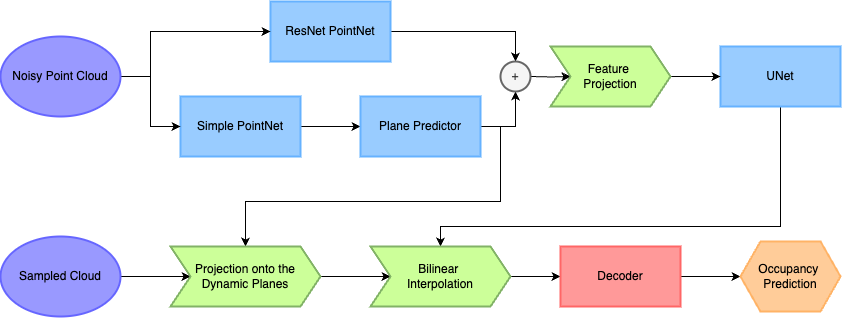
\includegraphics[width=\textwidth]{../media/pipeline_chiaro.png}
\end{frame}

\begin{frame}{Encoder}
The Encoder takes in input the Noisy Cloud and is composed by the following steps:
\begin{itemize}
\item ResNet PointNet
\item Simple PointNet + Plane Predictor 
\item Feature summation + projection 
\item UNet
\end{itemize}
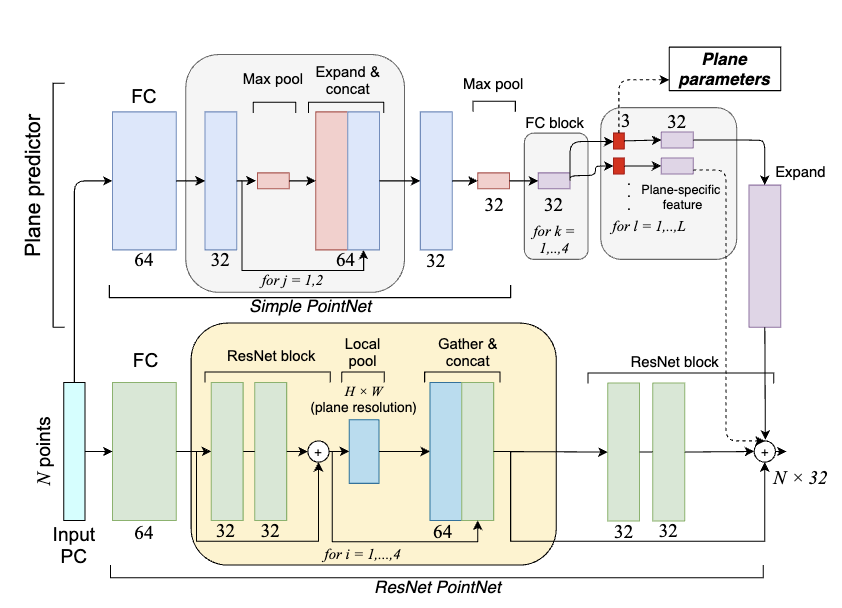
\includegraphics[width=\textwidth]{../media/encoder.png}
\end{frame}

\begin{frame}{Decoder}
The Dec is composed by:
\begin{itemize}
\item Feature Projection and Bilinear Interpolation
\item Occupancy Network
\end{itemize}
\end{frame}

\section{Reconstruction}

\begin{frame}{Multiresolution IsoSurface Extraction (MISE)}
    \begin{columns}[T]
      \column{0.5\textwidth}
        \begin{itemize}
            \item Create a grid over all the bounding box 
            \item Evaluate the occupancy of each corner of the voxels
            \item Define the Active voxels as the one composed with at least one occupied corner and one not 
            \item Subdivide each Active voxels into 8 subvoxels ($2x2x2$ grid) and evaluate the new points occupancy
            \item Repeat until the desired resolution is obtained
        \end{itemize}
      \column{0.5\textwidth}
        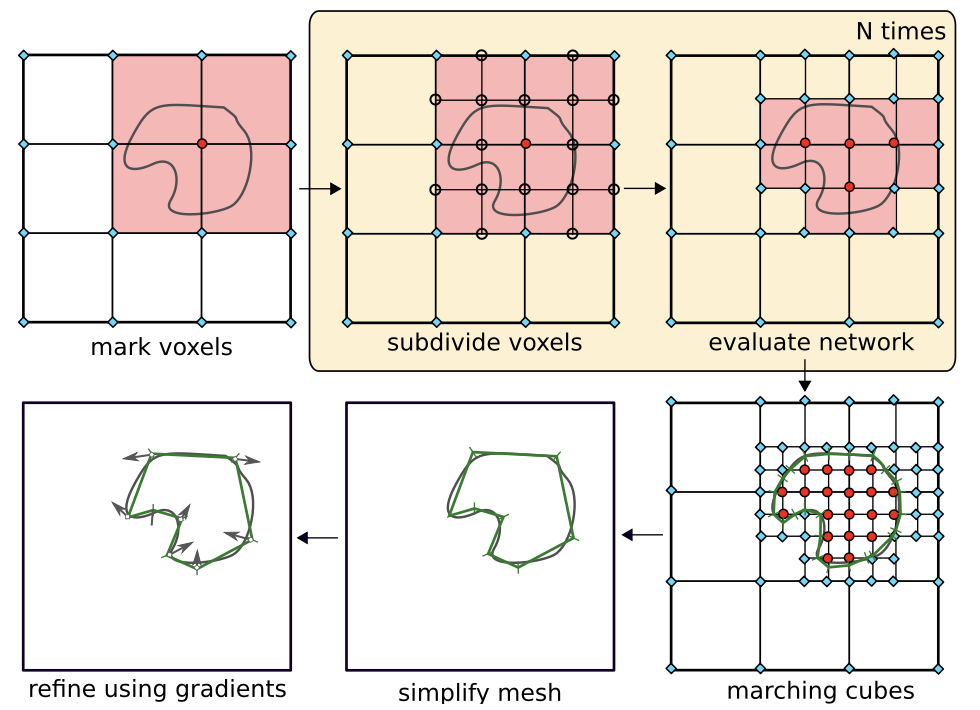
\includegraphics[width=\linewidth]{../media/mise.png}
    \end{columns}
  \end{frame}

\section{Results}

\begin{frame}{Metrics}
In order to evaluate the performance of our model, the following metrics have been used:
\begin{itemize}
\item Chamfer Distance : \\ 
$
CD(A, B) = \frac{1}{|A|} \sum_{a \in A} \min_{b \in B} \|a - b\|_2^2 + \frac{1}{|B|} \sum_{b \in B} \min_{a \in A} \|b - a\|_2^2
$
\item IOU : 
$ IoU(A', B') = \frac{|A' \cap B'|}{|A' \cup B'|}$
\item F-Score:
\end{itemize}
Add each formula
\end{frame}

\begin{frame}{Loss Performances}
Insert here plots
\end{frame}

\begin{frame}{Metrics Performances}
Insert here just a table with metrics, gpu usage
various types of sampling
\end{frame}

\section{Improvements}

\begin{frame}{Possible Changes and Future Improvements}
\end{frame}

\backmatter
\end{document}